\documentclass[10pt,aspectratio=169]{beamer}

\usetheme{metropolis}
\usepackage{appendixnumberbeamer}
\usepackage{booktabs}
\usepackage{tabularx}
\usepackage{graphicx}
\usepackage[french]{babel}
\usepackage{csquotes}

% Safer pdflatex support
\usepackage{iftex}
\ifPDFTeX
  \usepackage[T1]{fontenc}
  \usepackage[utf8]{inputenc}
  \DeclareUnicodeCharacter{00D7}{$\times$}
  \DeclareUnicodeCharacter{00B7}{\textperiodcentered}
\fi

% TikZ
\usepackage{tikz}
\usetikzlibrary{positioning, arrows.meta}

% Palette
\definecolor{mDarkTeal}{HTML}{1B2A41}
\definecolor{mLightBrown}{HTML}{F2A104}

% Safe logo command: if the logo file is missing, compilation still works
\newcommand{\safelogo}[2]{%
  \IfFileExists{#1}{%
    \includegraphics[height=1.05cm]{#1}%
  }{%
    \begin{tikzpicture}
      \node[
        draw=mDarkTeal!50,
        rounded corners=2pt,
        minimum width=1.9cm,
        minimum height=1.05cm,
        align=center,
        font=\scriptsize\bfseries,
        text=mDarkTeal
      ] {#2};
    \end{tikzpicture}%
  }%
}

\setbeamertemplate{frame numbering}[fraction]
\metroset{progressbar=frametitle,sectionpage=progressbar,numbering=fraction}

\title{Détection d'Anomalies et Diagnostic de Défauts dans les Systèmes Photovoltaïques par IA}
\subtitle{Déploiement sur Plateforme Embarquée Jetson Nano}
\author{GUERRAICHE Ahmed Amine \and MENASSEL Rayane Ibrahim}
\institute{ESI $\times$ CDER --- Projet de Fin d'Études 2025/2026 \\[2pt]
  \footnotesize Encadrants : Dr. DAHMANI Rabea (ESI) · Dr. RENNANE Ahmed, Dr. DALI Ali (CDER)}
\date{}

\begin{document}

% ════════════════════════════════════════════════════════════
% Page de garde
% ════════════════════════════════════════════════════════════
\begin{frame}[plain,noframenumbering]
  \centering
  \vspace*{0.5cm}

  \noindent
  \begin{minipage}[c]{0.16\textwidth}
    \centering\safelogo{../figures/logo_esi.png}{ESI}
  \end{minipage}%
  \hfill
  \begin{minipage}[c]{0.58\textwidth}
    \centering
    \colorbox{mDarkTeal}{\color{white}\textbf{\normalsize SOUTENANCE DE PROJET DE FIN D'ÉTUDES}}
  \end{minipage}%
  \hfill
  \begin{minipage}[c]{0.16\textwidth}
    \centering\safelogo{../figures/logo_cder.png}{CDER}
  \end{minipage}

  \vspace{1pt}
  {\small Pour l'obtention du Diplôme d'Ingénieur d'État en Informatique\par}
  \vspace{1pt}
  {\color{mDarkTeal!40}\rule{0.85\textwidth}{0.6pt}}
  \vspace{1pt}

  {\Large\bfseries\color{mDarkTeal}\inserttitle\par}
  \vspace{6pt}
  {\large\insertsubtitle\par}
  \vspace{7pt}

  \begin{columns}[T,onlytextwidth]
    \column{.5\textwidth}
      \centering
      {\small\textbf{Présenté par}}\\[4pt]
      GUERRAICHE Ahmed Amine\\
      MENASSEL Rayane Ibrahim
    \column{.5\textwidth}
      \centering
      {\small\textbf{Encadrants}}\\[4pt]
      Dr. DAHMANI Rabea (ESI)\\
      Dr. RENNANE Ahmed (CDER)\\
      Dr. DALI Ali (CDER)
  \end{columns}

  \vspace{3.5pt}
  {\small Promotion 2025/2026\par}
  \vspace*{0.45cm}
\end{frame}

\begin{frame}{Sommaire}
  \tableofcontents
\end{frame}

% ════════════════════════════════════════════════════════════
\section{Contexte et positionnement}
% ════════════════════════════════════════════════════════════

\begin{frame}{Du poster master à ce mémoire}
  \begin{columns}[T]
    \begin{column}{0.5\textwidth}
      \footnotesize
      \textbf{Hors ligne -- Machine Learning}
      \begin{itemize}
        \item \textbf{Noyau} (SVM, OC-SVM) -- Suliman et al. (2024) : SVM multi-noyau vs XGBoost adaptatif, 87,56\%
        \item \textbf{Ensembles} (RF, Isolation Forest) -- Amiri et al. (2024) : Random Forest, 99,4\% (détection + diagnostic)
      \end{itemize}
    \end{column}

    \begin{column}{0.48\textwidth}
      \textbf{Ce que ce mémoire construit}
      \begin{itemize}
        \item \textbf{Séquentiel} (LSTM, SSM, Transformer) -- Hajji et al. (2023) : BiLSTM, $\approx$100\% (simulé)
        \item \textbf{Reconstruction} (AE, VAE) -- Seghiour et al. (2023) : autoencodeur, 99,9\%
      \end{itemize}
    \end{column}
  \end{columns}
  \vfill
  \textbf{En ligne (streaming)} -- changepoint bayésien (BOCD), manifold régularisé, passive-aggressive : peu exploré côté PV malgré la compatibilité naturelle avec l'edge ; repris comme un des détecteurs évalués dans ce mémoire.
\end{frame}

% ════════════════════════════════════════════════════════════
\section{Etat de l'art}
% ════════════════════════════════════════════════════════════

\begin{frame}{Pourquoi la modalité électrique + météo}
  \begin{itemize}
    \item Imagerie thermique : coût élevé, sensibilité aux conditions ambiantes.
    \item Courbe I-V : nécessite souvent interruption de production, interprétation ambiguë.
    \item \alert{Électrique + météo} : mesures continues, infrastructure SCADA existante.
  \end{itemize}
\end{frame}

\begin{frame}{État de l'art --- données électriques \& météo}
\begin{columns}[T,onlytextwidth]

\column{0.49\textwidth}
\centering
\vspace{3pt}

\resizebox{\linewidth}{!}{%
\begin{tikzpicture}[
  edge from parent/.style={draw, -latex},
  every node/.style={font=\scriptsize, align=center},
  root/.style={
    fill=mDarkTeal!15,
    rounded corners,
    draw=mDarkTeal!50,
    inner sep=4pt
  },
  method/.style={
    fill=mLightBrown!20,
    rounded corners,
    draw=mLightBrown!70!black,
    inner sep=4pt,
    minimum width=24mm
  },
  refs/.style={
    font=\tiny,
    align=center,
    text width=26mm,
    inner sep=2pt
  },
  link/.style={draw, -latex, line width=0.3pt},
  refline/.style={draw, line width=0.25pt}
]

\node[root] (root) at (0,0) {Approches classiques};

\node[method] (svm) at (-2.8,-1.15) {SVM \& noyau};
\node[method] (rf)  at (0,-1.15) {Forêts\\aléatoires};
\node[method] (gb)  at (2.8,-1.15) {Boosting\\de gradient};

\node[refs, anchor=north] (svmrefs) at (-2.8,-1.75)
{Suliman et al. (2024)\\Cai \& Wai (2022)\\Saiprakash et al. (2024)};

\node[refs, anchor=north] (rfrefs) at (0,-1.75)
{Amiri et al. (2024b)};

\node[refs, anchor=north] (gbrefs) at (2.8,-1.75)
{Suliman et al. (2024)\\Noura et al. (2025)\\Kull et al. (2025)};

\draw[link] (root.south) -- ++(0,-0.18) -| (svm.north);
\draw[link] (root.south) -- ++(0,-0.18) -| (rf.north);
\draw[link] (root.south) -- ++(0,-0.18) -| (gb.north);

\draw[refline] (svm.south) -- (svmrefs.north);
\draw[refline] (rf.south) -- (rfrefs.north);
\draw[refline] (gb.south) -- (gbrefs.north);

\end{tikzpicture}
}

\column{0.49\textwidth}
\centering
\vspace{3pt}

\resizebox{\linewidth}{!}{%
\begin{tikzpicture}[
  edge from parent/.style={draw, -latex},
  every node/.style={font=\scriptsize, align=center},
  root/.style={
    fill=mDarkTeal!15,
    rounded corners,
    draw=mDarkTeal!50,
    inner sep=4pt
  },
  method/.style={
    fill=mLightBrown!20,
    rounded corners,
    draw=mLightBrown!70!black,
    inner sep=4pt,
    minimum width=24mm
  },
  refs/.style={
    font=\tiny,
    align=center,
    text width=28mm,
    inner sep=2pt
  },
  link/.style={draw, -latex, line width=0.3pt},
  refline/.style={draw, line width=0.25pt}
]

\node[root] (root) at (0,0) {Approches profondes};

\node[method] (rnn) at (-2.8,-1.15) {RNN\\LSTM, GRU};
\node[method] (ae)  at (0,-1.15) {Auto-\\encodeurs};
\node[method] (tr)  at (2.8,-1.15) {Transformers\\Graphes};

\node[refs, anchor=north] (rnnrefs) at (-2.8,-1.75)
{Hajji et al. (2023)\\Amiri et al. (2024a)};

\node[refs, anchor=north] (aerefs) at (0,-1.75)
{Seghiour et al. (2023)\\Titouni et al. (2025)\\Attouri et al. (2026)};

\node[refs, anchor=north] (trrefs) at (2.8,-1.75)
{Khalil et al. (2024)\\Balachandran et al. (2025)\\Yan et al. (2025)};

\draw[link] (root.south) -- ++(0,-0.18) -| (rnn.north);
\draw[link] (root.south) -- ++(0,-0.18) -| (ae.north);
\draw[link] (root.south) -- ++(0,-0.18) -| (tr.north);

\draw[refline] (rnn.south) -- (rnnrefs.north);
\draw[refline] (ae.south) -- (aerefs.north);
\draw[refline] (tr.south) -- (trrefs.north);

\end{tikzpicture}
}

\end{columns}
\end{frame}

\begin{frame}{Lacunes de recherche identifiées}
\centering

\vspace{0.2cm}

\begin{tikzpicture}[
  gapbox/.style={
    fill=mDarkTeal!10,
    draw=mDarkTeal!55,
    rounded corners=6pt,
    line width=0.5pt,
    text width=0.82\textwidth,
    align=left,
    inner xsep=10pt,
    inner ysep=8pt
  },
  icon/.style={
    circle,
    fill=mLightBrown!35,
    draw=mLightBrown!70!black,
    minimum size=7mm,
    font=\bfseries\small,
    text=mDarkTeal
  }
]

\node[gapbox] (g1) at (0,0) {
  \textbf{\color{mDarkTeal}Prédominance des jeux de données simulés}
};
\node[icon, left=4mm of g1] {1};

\node[gapbox, below=0.42cm of g1] (g2) {
  \textbf{\color{mDarkTeal}États défaillants difficiles à distinguer}
};
\node[icon, left=4mm of g2] {2};

\node[gapbox, below=0.42cm of g2] (g3) {
  \textbf{\color{mDarkTeal}Absence d'évaluation embarquée}
};
\node[icon, left=4mm of g3] {3};

\end{tikzpicture}

\end{frame}

% ════════════════════════════════════════════════════════════
\section{Conception}
% ════════════════════════════════════════════════════════════

\begin{frame}{Phases du processus FDD}

\centering
\vspace{0.4cm}

\begin{tikzpicture}[
  node distance=0.55cm,
  block/.style={
    draw=mDarkTeal!65,
    fill=mDarkTeal!8,
    rounded corners=4pt,
    minimum height=1.25cm,
    text width=0.20\textwidth,
    align=center,
    font=\scriptsize
  },
  arrow/.style={
    -{Latex[length=2mm]},
    draw=mDarkTeal!80,
    line width=0.5pt
  }
]

\node[block] (data) {
  \textbf{\color{mDarkTeal}Collecte \& transformation}
};

\node[block, right=of data] (detect) {
  \textbf{\color{mDarkTeal}Détection d'anomalies}
};

\node[block, right=1.15cm of detect] (diag) {
  \textbf{\color{mDarkTeal}Diagnostic}
};

\node[block, right=of diag] (monitor) {
  \textbf{\color{mDarkTeal}Interface de monitoring}
};

\draw[arrow] (data) -- (detect);
\draw[arrow] (detect) --
  node[above, font=\tiny, inner sep=1pt, yshift=2pt] {si anomalie}
  (diag);
\draw[arrow] (diag) -- (monitor);

\end{tikzpicture}

\end{frame}

\begin{frame}{Sélection du jeu de données}

\begin{block}{Dataset Costa}
\begin{itemize}
  \item Données réelles de terrain issues d'une installation photovoltaïque.
  \item Mesures électriques et météorologiques adaptées au FDD.
  \item Quatre défauts annotés : ombrage, dégradation, circuit ouvert et court-circuit.
  \item Volume important de données, exploitable pour l'apprentissage et l'évaluation.
\end{itemize}
\end{block}

\vspace{0.3cm}

\begin{block}{Intérêt pour notre travail}
\begin{itemize}
  \item Permet d'évaluer les modèles dans des conditions plus proches du réel.
  \item Compatible avec une approche de détection puis de diagnostic des défauts.
\end{itemize}
\end{block}

\end{frame}
\begin{frame}{Pipeline de données}

\centering
\vspace{0.4cm}

\resizebox{\textwidth}{!}{%
\begin{tikzpicture}[
  block/.style={
    draw=black,
    rounded corners=8pt,
    minimum width=3.2cm,
    minimum height=1.6cm,
    align=center,
    font=\normalsize\bfseries
  },
  arrow/.style={
    -{Latex[length=3mm]},
    line width=0.7pt
  },
  outlabel/.style={
    font=\small,
    align=center,
    text width=3.0cm
  }
]

\node[block] (ing)   at (0,0)    {Ingestion};
\node[block] (split) at (6.0,0)  {Découpage};
\node[block] (prep)  at (12.0,0) {Prétraitement};
\node[block] (feat)  at (18.0,0) {Extraction\\des caractéristiques};
\node[block] (train) at (24.0,0) {Entraînement};

\draw[arrow] (ing)   -- node[outlabel, below=8pt] {Table opérationnelle\\unifiée}          (split);
\draw[arrow] (split) -- node[outlabel, below=8pt] {Ensembles\\train / val / test}           (prep);
\draw[arrow] (prep)  -- node[outlabel, below=8pt] {Jeu de données\\nettoyé}                 (feat);
\draw[arrow] (feat)  -- node[outlabel, below=8pt] {Profils enrichis\\en caractéristiques}   (train);

\end{tikzpicture}
}

\end{frame}

\section{Implementation}



% ════════════════════════════════════════════════════════════
\section{Détection d'anomalies (Tâche A)}
% ════════════════════════════════════════════════════════════

\begin{frame}{Limite du binary PR-AUC}
  \footnotesize
  Le binary PR-AUC ne demande qu'une chose : distinguer \emph{une} panne, n'importe laquelle, du fonctionnement normal.
  \begin{table}
    \centering\footnotesize
    \begin{tabular}{l@{\hspace{1.2cm}}r}
      \toprule
      \textbf{Détecteur} & \textbf{Binary PR-AUC} \\
      \midrule
      \onslide<1->{BOCD} & \onslide<1->{0,870} \\
      \onslide<2->{Isolation Forest} & \onslide<2->{0,974} \\
      \onslide<3->{MAAT} & \onslide<3->{0,982} \\
      \onslide<4->{OC-SVM} & \onslide<4->{0,987} \\
      \onslide<5->{GTBAD} & \onslide<5->{0,9896} \\
      \onslide<6->{PC-Flow} & \onslide<6->{0,972} \\
      \bottomrule
    \end{tabular}
  \end{table}
  \onslide<7->{\scriptsize\alert{Cinq modèles sur six entre 0,97 et 0,99 -- presque tous \og excellents \fg{}.} Shadowing (35,7\% des lignes en panne) domine le calcul : un modèle qui n'attrape \emph{que} Shadowing score déjà très haut. PC-Flow termine \emph{dernier} des cinq modèles forts.}
\end{frame}

\begin{frame}{La révélation : macro PR-AUC}
  % TODO: S09
\end{frame}

\begin{frame}{Le cas de la classe Dégradation}
  \footnotesize
  Short-Circuit, Open-Circuit, Shadowing : tous les modèles compétitifs frôlent 1,0 -- signatures abruptes, faciles à séparer.
  \begin{table}
    \centering\footnotesize
    \begin{tabular}{l@{\hspace{1.2cm}}r}
      \toprule
      \textbf{Détecteur} & \textbf{PR-AUC -- Dégradation} \\
      \midrule
      \onslide<1->{BOCD} & \onslide<1->{0,121} \\
      \onslide<2->{Isolation Forest} & \onslide<2->{0,496} \\
      \onslide<3->{MAAT} & \onslide<3->{0,753} \\
      \onslide<4->{OC-SVM} & \onslide<4->{0,884} \\
      \onslide<5->{GTBAD} & \onslide<5->{0,914} \\
      \onslide<6->{\textbf{PC-Flow}} & \onslide<6->{\textbf{0,998}} \\
      \bottomrule
    \end{tabular}
  \end{table}
  \onslide<7->{\scriptsize\alert{La Dégradation est un défaut de contact à haute résistance, injecté de façon contrôlée} (et non une dérive d'usure naturelle) : chaque mesure isolée reste proche de la normale, sans événement net. PC-Flow score par \emph{probabilité conditionnelle} (irradiance, température), pas par magnitude d'erreur -- un écart discret par rapport à la variété physique attendue tombe dans la queue de faible probabilité même quand chaque signal a l'air ordinaire.}
\end{frame}

\begin{frame}{PC-Flow --- principe}
  Un \alert{normalizing flow} : un transport bijectif $f_\theta : \mathbb{R}^n \to \mathbb{R}^n$, $z = f_\theta^{-1}(x)$, exactement inversible.
  \begin{itemize}[<+->]
    \item Contrairement à un VAE (borne inférieure sur la vraisemblance), le flow donne une \alert{vraisemblance exacte} via le changement de variables :
    \[
      \log p(x;\theta) = \log p_Z\bigl(f_\theta^{-1}(x)\bigr) + \log\left|\det\frac{\partial f_\theta^{-1}(x)}{\partial x}\right|
    \]
    \item Architecture : conditional \texttt{RealNVP}, coupling layers affines, contexte $c = [\text{irradiance}, T_{\text{PV}}]$ injecté à chaque bloc
    \item Score d'anomalie = $-\log p(x \mid c;\theta)$ -- pas de feature engineering manuel requis
    \item \alert{Aucun travail antérieur} n'avait appliqué un normalizing flow à la détection de défauts PV
  \end{itemize}
\end{frame}

\begin{frame}{PC-Flow --- intuition géométrique}
  % TODO: S12
\end{frame}

\begin{frame}{Performance vs compacité}
  \footnotesize
  Le concurrent le plus proche, GTBAD, est statistiquement proche en macro PR-AUC -- mais pas en taille.
  \begin{table}
    \centering\footnotesize
    \begin{tabular}{l@{\hspace{1cm}}r@{\hspace{1cm}}r}
      \toprule
      \textbf{Détecteur} & \textbf{Macro PR-AUC} & \textbf{Paramètres} \\
      \midrule
      \onslide<1->{GTBAD} & \onslide<1->{0,9752~$\pm$~0,071} & \onslide<1->{869\,769} \\
      \onslide<2->{\textbf{PC-Flow}} & \onslide<2->{\textbf{0,990~$\pm$~0,005}} & \onslide<2->{\textbf{20\,124}} \\
      \bottomrule
    \end{tabular}
  \end{table}
  \onslide<3->{\alert{$43\times$ plus petit} pour un score égal ou supérieur. Sur Jetson Nano, mémoire et temps d'inférence croissent avec le nombre de paramètres -- c'est le facteur décisif pour la cible embarquée.}
\end{frame}

\begin{frame}{Calibration des seuils ISA-18.2}
  \footnotesize
  Trois opérateurs sur le \emph{même} score PC-Flow, calibrés uniquement sur les scores normaux d'entraînement -- chaîne d'escalade séquentielle P3~$\to$~P2~$\to$~P1 :
  \begin{table}
    \centering\footnotesize
    \begin{tabular}{l@{\hspace{0.6cm}}l@{\hspace{0.6cm}}r@{\hspace{0.6cm}}l}
      \toprule
      \textbf{Tier} & \textbf{Méthode} & \textbf{Précision} & \textbf{Rappel / Délai} \\
      \midrule
      \onslide<1->{P3 -- Advisory} & \onslide<1->{GPD/POT, FPR~$\leq$~20\%} & \onslide<1->{0,9174} & \onslide<1->{0,9167} \\
      \onslide<2->{P2 -- High} & \onslide<2->{Conformal, $\alpha=0,05$} & \onslide<2->{0,9705} & \onslide<2->{0,7050} \\
      \onslide<3->{P1 -- Critical} & \onslide<3->{CUSUM séquentiel} & \onslide<3->{1,0000} & \onslide<3->{63 échantillons} \\
      \bottomrule
    \end{tabular}
  \end{table}
  \onslide<4->{P3 favorise le rappel comme alerte précoce ; P2 garantit un FPR~$\leq$~5\% (distribution-free) ; P1 n'alarme que sur une dérive \emph{persistante}, au prix d'un délai médian de 63 échantillons.}
\end{frame}

% ════════════════════════════════════════════════════════════
\section{Diagnostic de défaults (Tâche B)}
% ════════════════════════════════════════════════════════════

\begin{frame}{Sélection du classifieur de pannes}
  \footnotesize
  3 ensembles d'arbres, 35 essais Optuna TPE chacun, objectif macro F1, sur le profil \texttt{plus\_physics} :
  \begin{table}
    \centering\footnotesize
    \begin{tabular}{l@{\hspace{0.6cm}}r@{\hspace{0.6cm}}r@{\hspace{0.6cm}}l}
      \toprule
      \textbf{Modèle} & \textbf{Macro F1} & \textbf{Bal.\ Acc.} & \textbf{Worst-class F1} \\
      \midrule
      \onslide<1->{LightGBM} & \onslide<1->{0,934~$\pm$~0,098} & \onslide<1->{0,925~$\pm$~0,131} & \onslide<1->{0,860 (Dégrad.)} \\
      \onslide<2->{CatBoost} & \onslide<2->{0,948~$\pm$~0,090} & \onslide<2->{0,932~$\pm$~0,124} & \onslide<2->{0,893 (Dégrad.)} \\
      \onslide<3->{\textbf{ExtraTrees}} & \onslide<3->{\textbf{0,959~$\pm$~0,078}} & \onslide<3->{\textbf{0,943~$\pm$~0,113}} & \onslide<3->{\textbf{0,922}} \\
      \bottomrule
    \end{tabular}
  \end{table}
  \onslide<4->{ExtraTrees l'emporte sur \emph{tous} les critères avec le plus faible écart entre folds. Son double aléa (features \emph{et} seuils) agit comme régularisateur naturel -- précieux quand les classes minoritaires comptent très peu d'épisodes (15--23).}
  \onslide<5->{\footnotesize \texttt{voltage\_imbalance} (41\%) et \texttt{pdc\_temp\_corrected} (16\%) dominent l'importance des features -- la feature engineering physique se valide elle-même.}
\end{frame}

\begin{frame}{Calibration des probabilités}
  \footnotesize
  Les scores bruts d'ExtraTrees ne sont pas garantis calibrés : confiance de 0,9 $\neq$ 90\% de fiabilité réelle. Recalibration par \texttt{Platt scaling} (sigmoïde, fit sur validation) :
  \begin{table}
    \centering\footnotesize
    \begin{tabular}{l@{\hspace{1.2cm}}r}
      \toprule
      \textbf{Métrique (test, calibré)} & \textbf{Valeur} \\
      \midrule
      \onslide<1->{Log-loss} & \onslide<1->{0,059} \\
      \onslide<2->{Brier score} & \onslide<2->{0,008} \\
      \onslide<3->{ECE} & \onslide<3->{0,019} \\
      \onslide<4->{MCE} & \onslide<4->{0,754} \\
      \bottomrule
    \end{tabular}
  \end{table}
  \onslide<5->{Log-loss et Brier confirment un bon alignement global ; l'ECE de 0,019 montre une faible erreur \emph{moyenne}. Le MCE (effet de bin extrême, cf.\ Annexe~E) capture le pire cas, pas la qualité moyenne -- la confiance affichée à l'opérateur reste fiable dans l'ensemble.}
\end{frame}


\section{Déploiment}
\begin{frame}{Plateforme embarquée : NVIDIA Jetson Nano}

\begin{columns}[T,onlytextwidth]

\column{0.42\textwidth}
\centering
\vspace{0.3cm}

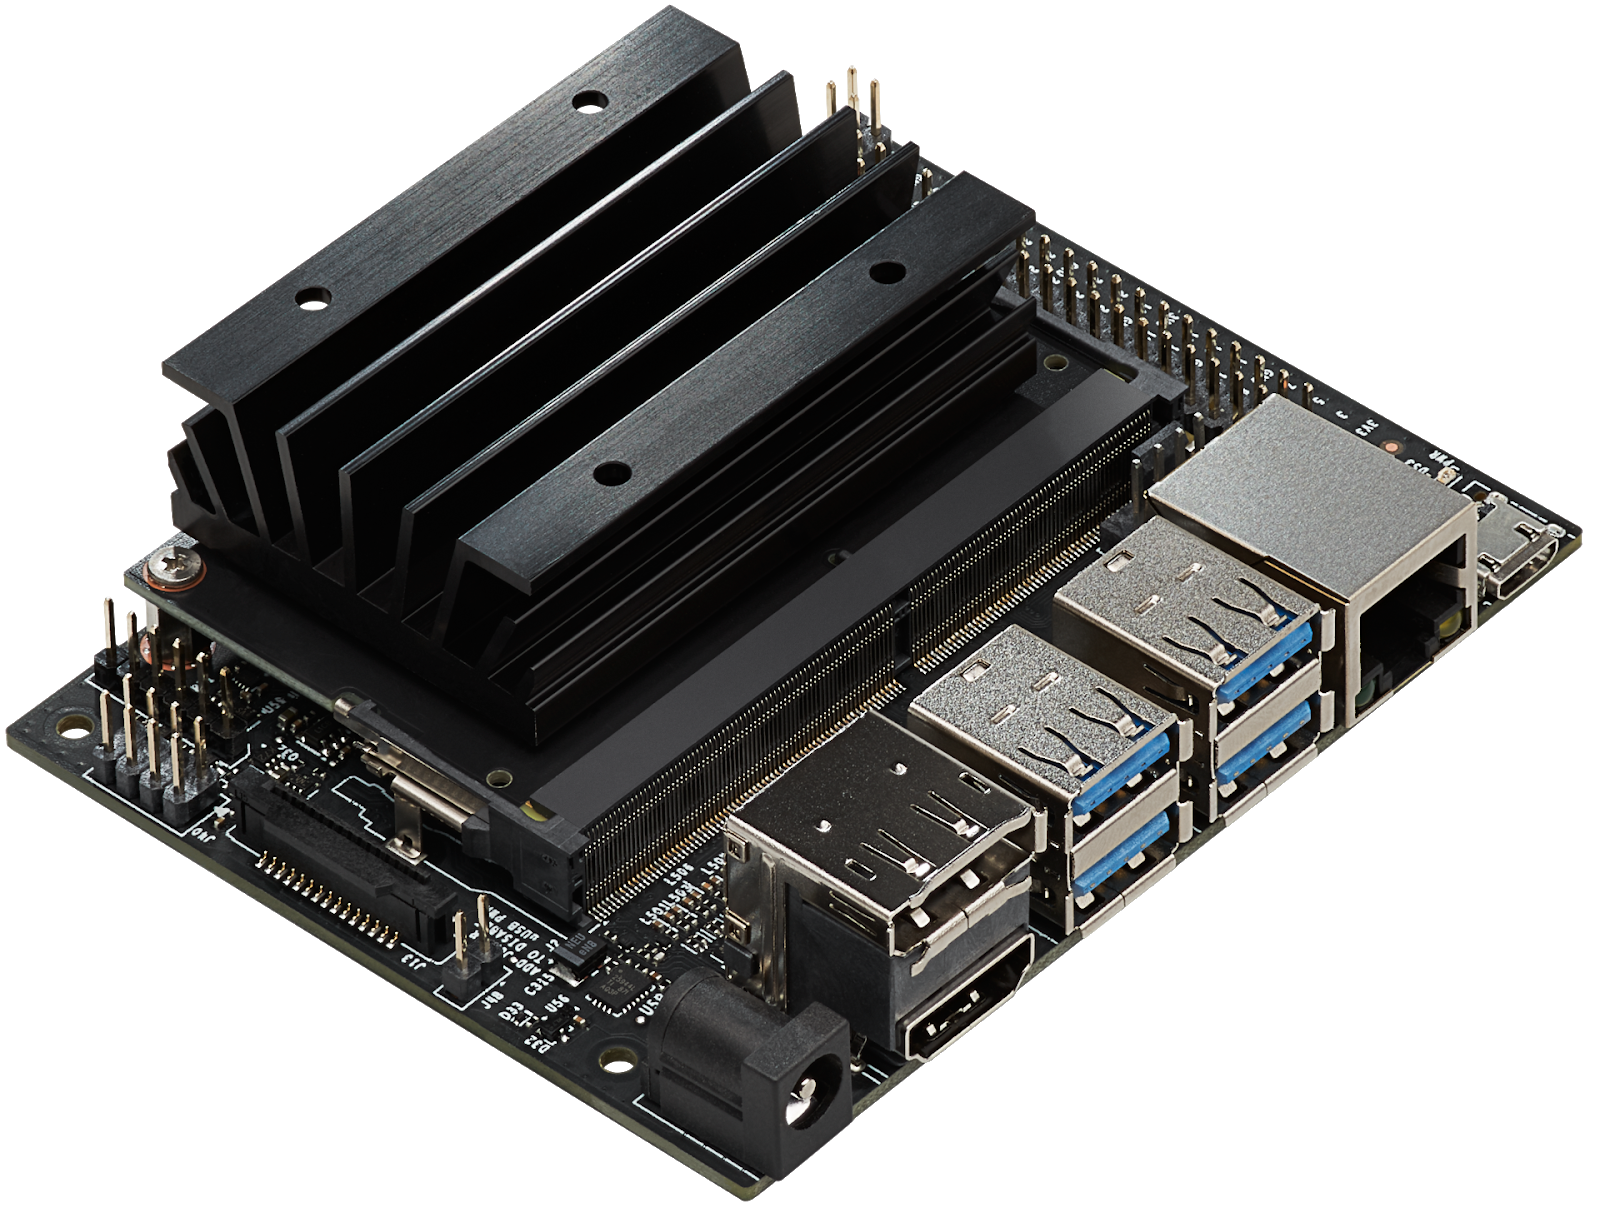
\includegraphics[
  width=0.9\linewidth
]{../figures/jetson-nano.png}

\vspace{0.15cm}
{\scriptsize NVIDIA Jetson Nano Developer Kit}

\column{0.55\textwidth}

\begin{block}{Caractéristiques principales}
\begin{itemize}
  \item Plateforme edge AI compacte et basse consommation.
  \item GPU NVIDIA Maxwell intégré pour l'accélération matérielle.
  \item Mémoire LPDDR4 suffisante pour des modèles légers.
  % \item Connectivité Ethernet et USB pour l'intégration avec capteurs et interfaces.
  \item Environnement JetPack avec CUDA, cuDNN et TensorRT.
\end{itemize}
\end{block}

\end{columns}

\end{frame}

\begin{frame}{Latence du système complet sur Jetson Nano}

\begin{block}{Protocole de mesure}
\begin{itemize}
  \item Rejeu de 162\,453 échantillons PV réels.
  \item Mesure du temps de traitement par échantillon sur la Jetson Nano.
  \item Budget temps réel : 1000 ms par échantillon.
\end{itemize}
\end{block}

\vspace{0.35cm}

\centering
\begin{tabular}{lccc}
\toprule
\textbf{Étape} & \textbf{p50} & \textbf{p95} & \textbf{p99} \\
\midrule
Détecteur PC-Flow & 8.97 ms & 13.58 ms & 19.04 ms \\
Classifieur ExtraTrees & 5.10 ms & 9.50 ms & 14.75 ms \\
\textbf{Pipeline complet} & \textbf{12.94 ms} & \textbf{21.44 ms} & \textbf{30.04 ms} \\
\bottomrule
\end{tabular}

\vspace{0.45cm}

\begin{block}{Résultat clé}
\vspace{0.1cm}

\centering
\small
Le pipeline complet reste largement sous la contrainte temps réel, avec une marge d'environ
\textbf{33$\times$ au 99\textsuperscript{e} centile}.
\end{block}

\end{frame} 

\begin{frame}{Détection de dérive opérationnelle}

\begin{block}{Objectif}
\begin{itemize}
  \item Vérifier que les conditions de déploiement restent proches du domaine vu à l'entraînement.
  \item Signaler une dérive avant qu'elle ne dégrade silencieusement la qualité de détection.
\end{itemize}
\end{block}

\vspace{0.25cm}

\begin{block}{Principe implémenté}
\begin{itemize}
  \item Surveillance du régime d'exploitation : irradiance et température PV $(irr, T_{PV})$.
  \item Agrégation quotidienne pour distinguer une dérive persistante du cycle jour/nuit.
  \item Test Page-Hinkley bidirectionnel pour détecter les changements de distribution.
\end{itemize}
\end{block}

\vspace{0.25cm}

\begin{block}{Niveaux de dérive}
\begin{itemize}
  \item \textbf{Normal} : aucune dérive détectée.
  \item \textbf{Advisory} : dérive persistante pendant 7 jours consécutifs.
  \item \textbf{Action-ready} : dérive persistante pendant 14 jours consécutifs.
\end{itemize}
\end{block}

\end{frame}
\begin{frame}{Architecture du module de monitoring}

\centering
\vspace{0.2cm}

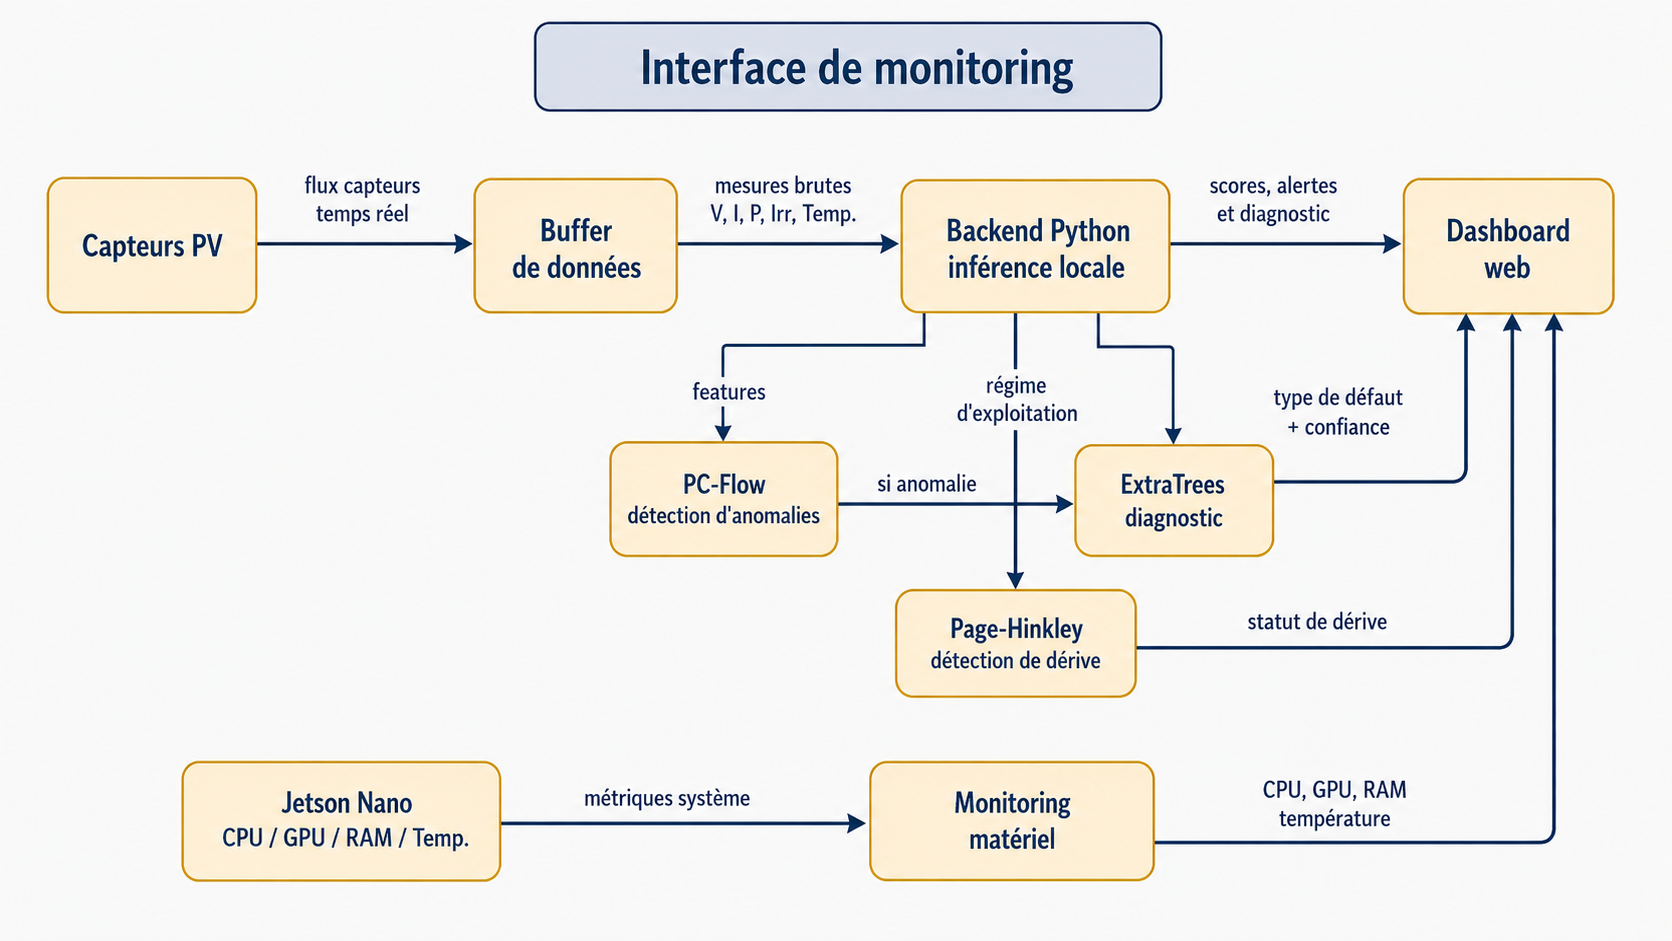
\includegraphics[
  width=0.98\textwidth,
  height=0.82\textheight,
  keepaspectratio
]{../figures/monitoring-arch.png}

\end{frame}

% -------------------- Slide 1: Conclusion --------------------
\begin{frame}{Conclusion --- résultats atteints}

\begin{block}{Système FDD complet}
\begin{itemize}
  \item Pipeline bout-en-bout : ingestion, découpage temporel, prétraitement et caractéristiques informées par la physique.
  \item Détection d'anomalies par PC-Flow, modèle compact et conditionné par le régime d'exploitation.
  \item Diagnostic des défauts par ExtraTrees avec pondération des classes.
  \item Déploiement embarqué sur Jetson Nano avec export ONNX et interface de monitoring.
\end{itemize}
\end{block}

\vspace{0.25cm}

\begin{block}{Résultats clés}
\begin{itemize}
  \item PC-Flow : PR-AUC binaire de \(0.989 \pm 0.008\), avec moins de 25\,000 paramètres.
  \item ExtraTrees : macro F1 de \(0.959 \pm 0.078\) et balanced accuracy de \(0.943 \pm 0.113\).
  \item Pipeline complet : exécution temps réel sur Jetson Nano avec une marge de \(33\times\) au 99\textsuperscript{e} centile.
\end{itemize}
\end{block}

\end{frame}


% -------------------- Slide 2: Limitations --------------------
\begin{frame}{Limites du système}

\begin{block}{Limites liées aux données}
\begin{itemize}
  \item Évaluation réalisée sur un seul dataset.
  \item Défauts induits dans des conditions contrôlées, donc généralisation terrain encore limitée.
  \item Couverture limitée à quatre classes seulement.
\end{itemize}
\end{block}

\vspace{0.25cm}

\begin{block}{Limites opérationnelles}
\begin{itemize}
  \item Campagne d'acquisition courte, sans cycle annuel complet contenant les variations saisonnières.
  \item Hypothèse d'un seul défaut dominant par fenêtre d'observation.
\end{itemize}
\end{block}

\end{frame}


% -------------------- Slide 3: Future perspectives --------------------
\begin{frame}{Perspectives futures}

\begin{block}{Données et validation}
\begin{itemize}
  \item Étendre l'évaluation à plusieurs sites PV et conditions climatiques.
  \item Collecter des défauts plus variés, avec différents niveaux de sévérité.
  \item Valider la robustesse sur des campagnes longues couvrant les variations saisonnières.
\end{itemize}
\end{block}

\vspace{0.25cm}

\begin{block}{Évolution du système}
\begin{itemize}
  \item Étudier le diagnostic multi-défauts pour les scénarios de pannes simultanées.
  \item Renforcer l'adaptation aux dérives par des mécanismes de recalibration ou de mise à jour.
  \item Enrichir l'interface opérateur avec des indicateurs d'explicabilité et d'aide à la décision.
\end{itemize}
\end{block}

\end{frame}


% -------------------- Slide 4: Thank you --------------------
\begin{frame}[plain,noframenumbering]
\begin{tikzpicture}[remember picture,overlay]
  % Background covers the entire physical page, not just the text area
  \fill[mDarkTeal] (current page.south west) rectangle (current page.north east);

  % Text centered exactly on the page (immune to beamer margins)
  \node[align=center] at (current page.center) {
    \sffamily\color{white}\Huge\bfseries Merci pour votre attention\\[0.4cm]
    % \sffamily\color{white!85!black}\Large\normalfont Place à la démonstration
  };
\end{tikzpicture}
\end{frame}
% ════════════════════════════════════════════════════════════
\appendix
\metroset{sectionpage=none}
\section{Annexes}
% ════════════════════════════════════════════════════════════

\begin{frame}{Annexe A --- Pourquoi Costa}
  \footnotesize
  \begin{table}
    \centering\scriptsize
    \begin{tabular}{l@{\hspace{0.5cm}}l@{\hspace{0.5cm}}l@{\hspace{0.5cm}}l}
      \toprule
      \textbf{Dataset} & \textbf{Origine} & \textbf{Taux} & \textbf{Classes / Météo} \\
      \midrule
      \onslide<1->{\textbf{Costa}} & \onslide<1->{Réel, terrain} & \onslide<1->{1~Hz} & \onslide<1->{4 pannes, Irr + T} \\
      \onslide<2->{La Réunion} & \onslide<2->{Réel, terrain} & \onslide<2->{$\approx$7~s} & \onslide<2->{7 (ombrage), météo compl.} \\
      \onslide<3->{GPVS-Faults} & \onslide<3->{Expérimental} & \onslide<3->{100~kHz} & \onslide<3->{7, aucune météo} \\
      \onslide<4->{Simulés (divers)} & \onslide<4->{Synthétique} & \onslide<4->{---} & \onslide<4->{idéalisés, peu de bruit} \\
      \bottomrule
    \end{tabular}
  \end{table}
  \onslide<5->{Costa : seul dataset réel à 1~Hz combinant 4 pannes électriques distinctes \emph{et} contexte météo (irradiance + température) -- condition nécessaire au conditionnement physique de PC-Flow.}
\end{frame}

\begin{frame}{Annexe B --- Justification du macro PR-AUC}
  \footnotesize
  \[
    \mathrm{PR\text{-}AUC}_{\mathrm{macro}} = \frac{1}{K}\sum_{k=1}^{K} \mathrm{PR\text{-}AUC}_k, \qquad K = 4
  \]
  \begin{itemize}[<+->]
    \item Le binary PR-AUC pondère implicitement par la fréquence -- Shadowing (35,7\% des lignes en panne) domine le calcul
    \item Le macro PR-AUC donne un poids \alert{égal} à chaque classe, indépendamment de sa fréquence
    \item Une panne rare (Short-Circuit, 15 épisodes) compte autant qu'une panne fréquente (Shadowing, 1000 épisodes)
    \item Cohérent avec l'objectif opérationnel : un détecteur aveugle à une panne rare reste inacceptable même s'il excelle sur la panne fréquente
  \end{itemize}
\end{frame}

\begin{frame}{Annexe C --- HPO PC-Flow}
  \footnotesize
  35 essais Optuna TPE, profil \texttt{baseline\_raw} :
  \begin{table}
    \centering\scriptsize
    \begin{tabular}{l@{\hspace{0.8cm}}l@{\hspace{0.8cm}}r}
      \toprule
      \textbf{Paramètre} & \textbf{Plage} & \textbf{Valeur retenue} \\
      \midrule
      \onslide<1->{\texttt{learning\_rate}} & \onslide<1->{$[10^{-4},10^{-2}]$ log-unif.} & \onslide<1->{$1{,}96\times10^{-4}$} \\
      \onslide<2->{\texttt{weight\_decay}} & \onslide<2->{$[10^{-6},10^{-3}]$ log-unif.} & \onslide<2->{$1{,}26\times10^{-5}$} \\
      \onslide<3->{\texttt{n\_coupling\_layers}} & \onslide<3->{$\{2,\ldots,6\}$} & \onslide<3->{4} \\
      \onslide<4->{\texttt{hidden\_dim}} & \onslide<4->{$\{32,64,128\}$} & \onslide<4->{64} \\
      \onslide<5->{\texttt{dropout}} & \onslide<5->{$[0,0{,}3]$} & \onslide<5->{0,0093} \\
      \bottomrule
    \end{tabular}
  \end{table}
\end{frame}

\begin{frame}{Annexe D --- Ablations PC-Flow}
  \footnotesize
  \begin{itemize}[<+->]
    \item \textbf{Profil de features} : macro PR-AUC se dégrade de 0,990 (7 features) à 0,955 (153 features, \texttt{plus\_rolling}) -- malédiction de la dimensionnalité ; le flow apprend déjà sa propre représentation
    \item \textbf{Conditionnement physique} : retirer irradiance/température fait chuter 0,985~$\to$~0,977 et double quasiment la variance (0,012~$\to$~0,021)
    \item \textbf{Scoring} : NLL affine (déployé, 0,985) bat spline-typicality (0,937) en macro PR-AUC, malgré un binary PR-AUC légèrement supérieur pour ce dernier (0,979 vs 0,964)
  \end{itemize}
\end{frame}

\begin{frame}{Annexe E --- MCE = 0,754, explication}
  \footnotesize
  \begin{itemize}[<+->]
    \item Le MCE capture l'écart \alert{pire-cas} entre confiance prédite et exactitude observée, sur un seul bin de confiance
    \item À ne pas confondre avec l'ECE (0,019), qui moyenne cet écart sur \emph{tous} les bins, pondéré par leur population
    \item Le bin concerné est un bin de très haute confiance et de très faible population (\og tail-bin effect \fg) -- quelques échantillons mal classés y suffisent à produire un grand écart relatif
    \item Log-loss (0,059) et Brier (0,008) confirment que la qualité \emph{globale} de calibration reste excellente
  \end{itemize}
\end{frame}

\begin{frame}{Annexe F --- Protocole de Drift opérationnel}
  \footnotesize
  Test \texttt{Page-Hinkley} bidirectionnel sur les statistiques journalières du régime opératoire $(\mathrm{irr}, T_{PV})$ :
  \[
    M_t = \sum_{i=1}^{t}(x_i - \bar{x} - \delta), \quad \mathrm{PH}_t = M_t - \min_{j\le t} M_j, \quad \text{drift} = \mathbf{1}[\mathrm{PH}_t > \lambda]
  \]
  \begin{itemize}
    \item Agrégation \alert{journalière} : distingue le drift saisonnier persistant du cycle diurne attendu
    \item Stade \textbf{advisory} après 7 jours consécutifs de glissement
    \item Stade \textbf{action-ready} après 14 jours consécutifs
    \item Surveille le \emph{régime}, indépendamment du score du modèle -- évite la circularité (cf.\ feedback circularité \& gates)
  \end{itemize}
\end{frame}

\begin{frame}{Annexe G --- HPO ExtraTrees \& leakage suite}
  \footnotesize
  \begin{columns}[T]
    \begin{column}{0.5\textwidth}
      \textbf{HPO (35 essais, macro F1)}
      \begin{itemize}[<+->]
        \item \texttt{n\_estimators} = 800
        \item \texttt{criterion} = entropy
        \item \texttt{max\_depth} = 24
        \item \texttt{max\_features} = 0,8
        \item \texttt{bootstrap} = True
      \end{itemize}
    \end{column}
    \begin{column}{0.5\textwidth}
      \textbf{Suite anti-leakage}
      \begin{itemize}[<+->]
        \item Label-shuffle macro F1 : 0,234 ($\approx$chance, 0,25)
        \item Top feature importance : 0,415, pas de proxy dominant
        \item Time-split \& duplicate check : conformes
      \end{itemize}
    \end{column}
  \end{columns}
\end{frame}

\end{document}